\chapter{s--d-model}\label{ch:sdmodel}
\section{Introduction}
Our model consists of two parts. The first part are the conducting electrons who's Hamiltonian is given by a tight-binding model. These conducting electrons can scatter of impurities in the material leading to having a finite momentum life-time. At the same time the spin of the electrons are coupled to its momentum through spin-orbit interactions, making it possible to transfer this angular momentum to the crystal lattice. The second part is the (anti)ferromagnet which we describe using a Heisenberg model in a classical limit, meaning we replace the spin-operators with vectors. In order to transfer angular momentum between localized and itinerant electrons, we therefore need to introduce a parameter that couples the spin and magnetic moment locally. This allows us to directly relate the relaxation of the momentum of itinerant electrons to the relaxation of angular momentum of the localized electrons. This momentum relaxation is at the heart of quantum transport theory. This model has much in comparison with the s--d model, used for example in the Kondo effect \cite{kondo}, where localized $d$ electrons are coupled to itinerant $s$ electrons. In the literature therefore our model is often called s--d, or s--d-like, and the parameter that couples the spins of localized and itenerant electrons is called an s--d-like exchange interaction. 

\section{Classical equations of motion on magnetization}
The Hamiltonian describing the localized and intenerant electrons is given by
\begin{multline}
    \hat{H}
        = \sum_{\mathclap{\{i,j\}\in\text{n.n.}}}\,\Big(\frac{J_{\text{ex}}}{n}\hat{\bb{S}}_i\cdot\hat{\bb{S}}_j - \frac{K}{2n}\hat{\bb{S}}_{z,i}\cdot\hat{\bb{S}}_{z,j}-t \hat{c}_i^\dagger\hat{c}_j\\
        -\lambda i c_i^\dagger \bb{u}_{ij}\cdot\bb{\sigma}\hat{c}_j\Big)+\sum_i \hslash\gamma_0\bb{H}_\text{ext}\cdot\hat{\bb{S}}_i-\Delta_\text{sd}\hat{\bb{S}}_i\cdot\hat{c}_i^\dagger\bb{\sigma}\hat{c}_i,
    \label{intro:eq:Hm}
\end{multline}
with the Heisenberg exchange energy $J_{\text{ex}}$, anisotropy constant $K$, s--d-like exchange energy $J_{\text{sd}}$, creation operators for itinerant electrons and localized spins $\hat{c}^\dagger_l$ and $\hat{S}$ respectively, Pauli-matrices $\bb{\sigma}$, external magnetic field $\bb{H}_\text{ext}$, gyromagnetic ratio $\gamma_0=|\gamma_0|$, hopping parameter $t$ and Rashba-spin-orbit $\lambda$, and $\bb{u}_{ij}$ is a vector that connects nearest neighbors at sites $i$ and $j$.  The first sum is taken over nearest neighbor sites. Note that the constant $K$ is inserted here phenomenologically, but can be computed as done later in Chapter~\ref{?} for a honeycomb antiferromagnet.

To describe the full dynamics of the system we assume that the expectation value of the localized spins move on a much larger time-scale than the spin-polarization of the conducting electrons. This allows us to decouple the system in two parts. We first derive equations of motion for the localized spins in a classical, mean-field approach by using only the expectation value of conducting electrons spin-polarization. Second, the spin-polarization of the conducting electrons is computed microscopically using linear response theory in response to electric currents and time-derivative of magnetizations, where the localized spins enter as classical fields. 

The mean-field approach simply constitutes the replacement
\begin{equation}
    \sum_{\mathclap{\{ij\}\in\text{n.n.}}} \bb{S}_i\cdot\bb{S}_j\rightarrow n\langle\bb{S}_j\rangle\cdot\sum_i \bb{S}_i
\end{equation}
with $n \langle \bb{S}_j\rangle$ the effective field produced by the $n$ nearest neighbors felt by $\bb{S}_i$. When $J_\text{ex}<0$, the spins favour parallel alignment and the energy can be written as
\begin{equation}
    E = \sum_{i} \Big(\mu_0 \hat{\bb{S}}_i\cdot \bb{H}_{\text{ext}}
    - K(\hat{S}_{z,i})^2)
    -J_{\text{sd}}\big(\bb{S}_i\cdot\bb{s}\big)
        \Big)
        \label{intro:eq:E1}
\end{equation}
where we introduced the spin polarization density $\bb{s} = \mathcal{A}^{-1}\langle \hat{c}^\dagger \bb{\sigma}\hat{c}\rangle$ (with unit cell area $\mathcal{A}$). In the case when $J_\text{ex}>0$ the spins favor antiparallel alignment and the energy can be written as
\begin{equation}
    E = \sum_{i} \Big(J_{\text{ex}}\bb{S}^\text{A}_i\cdot\bb{S}^\text{B}_i 
    - K((\hat{S}_{z,i}^\text{A})^2+(\hat{S}_{z,i}^\text{B})^2)
    -J_{\text{sd}}\big(\bb{S}^\text{A}_i\cdot\bb{s}^\text{A}+\bb{S}^\text{B}_i\cdot\bb{s}^\text{B}\big)
        \Big)
        \label{intro:eq:E2}
\end{equation}
where we introduced the spin polarization density $\bb{s}^\text{A(B)} = \mathcal{A}^{-1}\langle \hat{c}^\dagger \bb{\sigma}\hat{c}\rangle$ (with unit cell area $\mathcal{A}$). 

The equations of motion is given by $\partial_t \bb{S}_i = \{E,\bb{S}_i\}_p$, where $\{\cdots\}_p$ is the Poisson bracket. For angular momenta we simply have $\{\hslash \bb{S}_i,\hslash \bb{S}_j\}_p=\hslash \bb{S}_i\times\bb{S}_j$. As is common practice, the magnetization in the ferromagnet is expressed in terms of a unit vector $\bb{m} = -\bb{S}/|\bb{S}|$ and for an antiferromagnet we introduce the magnetization $\bb{m}$ and staggered magnetization (also called the Neel vector) $\bb{n}$ as
\begin{align}
 	\bb{m}&=-1/2(\bb{S}^\text{A}/|\bb{S}^\text{A}|+\bb{S}^\text{B}/|\bb{S}^\text{B}|)\\
    \bb{n}&=-1/2(\bb{S}^\text{A}/|\bb{S}^\text{A}|-\bb{S}^\text{B}/|\bb{S}^\text{B}|).
\end{align} 
With these considerations we find the following equations of motion of magnetization for a ferromagnet
\begin{align}
	\hslash \partial_t \bb{m} &= \bb{m}\times\big(-\hslash\gamma_0\bb{H}_\text{ext}+Km_z+\Delta_\text{sd}\bb{s}\big)
	\label{intro:eq:S1}
\end{align}
and the following for an antiferromagnet
\begin{align}
\hslash \partial_t \bb{n} =& -2J_\text{ex}\, \bb{n}\!\times\!\bb{m} \nonumber\\
    & + K \big(\bb{m}\!\times\!\bb{n}_\perp+\bb{n}\times\bb{m}_\perp\big) 
	+ \Delta_\text{sd} \big(\bb{m}\times\bb{s}^-+\bb{n}\times\bb{s}^+) -\hslash\gamma_0\bb{n}\times\bb{H}_\text{ext},\\
\hslash \partial_t \bb{m} =&K  \big(\bb{n}\!\times\!\bb{n}_\perp+\bb{m}\times\bb{m}_\perp\big) 
	+ \Delta_\text{sd} \big(\bb{m}\times\bb{s}^++\bb{n}\times\bb{s}^-)-\hslash\gamma_0\bb{m}\times\bb{H}_\text{ext}
	\label{eq:sd:neel}
\end{align}

The same equations of motion can be obtained by first using Heisenberg's equations of motion $i \hslash\partial_t \hat{S}_\alpha = [H,\hat{S}_\alpha]$ (where $\alpha=x,y,z$) and the commutation relations for spin-operators $[\hat{S}_x, \hat{S}_y]=i\hat{S}_z$ on Eq~(\ref{intro:eq:Hm}), and then taking the classical limit $\hat{\bb{S}}\rightarrow \bb{S}$. 

Note that the minus in front of the definitions of $\bb{n}$ and $\bb{m}$ are there because for electrons their magnetic moment is directed in opposite direction of their spin angular moment. Furthermore, although we use the same notation $\bb{m}$ for the magnetization in a ferro and anti-ferromagnet, it is only a unit-vector in the former case and not the latter. 

\section{Spin-torques}
The dynamics of the magnetization vector in ferromagnets and antiferromagnets are determined by spin-torques. In order to compute a spin-torque, all we need to do is compute the spin-density of the conducting electrons, which is done using linear response theory (see the next section).  
 These torques can be divided into two groups: field-like and damping-like. For antiferromagnets each group can be further subdivided into two: staggered and non-staggered. In a two-dimensional ferromagnet with spin-orbit of Rashba type, the equations of motion are often written phenomenologically as
\begin{equation}
    \partial_t \bb{m} = c_1 \bb{m}\times (\hat{\bb{z}}\times\bb{j}) + c_2 \bb{m}\times\big(\bb{m}\times (\hat{\bb{z}}\times{j})\big) + \alpha \bb{m}\times \partial_t \bb{m},
    \label{eq:sd:ferro}
\end{equation}
where the terms proportional to $c_1$ and $c_2$ are torques that are induced by injecting an electric current $\bb{j}$ and the term proportional to $\alpha$ describes the rate of dissipation of angular momentum and is called Gilbert damping. The field-like and damping-like torques can be identified as those that are respectively even and odd under time-reversal (i.e. changing the signs of $\bb{m}$, $\bb{j}$ and $t$). Note that the spin of the conducting electrons must be odd in time-reversal, so that applying time-reversal on both the magnetic subsystem and the tightbinding model, one will find that the coefficients $c_1$ and $c_3$ are even, while $c_2$ must be odd under total time-reversal. Note that by symmetry we must have that $c_1$ and $\alpha$ are even in scattering time, while $c_2$ is odd in scattering time. In the literature dealing with microscopic theory there is a substantial lack of damping-like torques. The reason is that is it not easy to make $c_2$ odd in scattering time. Since in the current density $\bb{j}$ is already linear in scattering time, one either needs to go beyond linear response or find less trivial mechanisms for the relaxation of angular momentum. For example, we will see in Chapter~\ref{ch:summit} that an damping-like torque appears when the Fermi surface becomes anisotropic. 

Distinguising between field-like and damping-like torques helps us understand more the dynamics of $\bb{n}$. For example, if the damping-like torques are absent one will only observe a simple precession of the magnetization vector around $\hat{\bb{z}}\times\bb{j}$. Damping-like torques allow for the dissipation of angular momentum so that over time the magnezation vector will be parallel to $\hat{\bb{z}}\times\bb{j}$. The dynamics induced by both field-like and damping-like torques are illustrated in Figure~\ref{fig:dynamics}. Note that we can change the sign of the damping-like torque by changing the direction of the electric current. If this current-induced damping-like torque overcomes the Gilbert damping one can even reverse the magnetization direction. In such a way one can construct a magnetic memory that stores a "0" or a "1" corresponding to two magnetization directions. This type of switching is illustrated in Figure~\ref{fig:switching}. The switching rate is determined by the strength of the damping-like torque which is proportional to Rashba spin-orbit coupling. It is then no surprise that putting a magnetic layer on top of a heavy metal will enhance its magnetic switching abilities. 

In an antiferromagnet we are more interested in the dynamics of $\bb{n}$. A phenomenological equation such as Eq.~(\ref{eq:sd:ferro}) can quickly contain ten terms for a antiferromagnet and the dynamics therefore is far more complicated. However, few points can still be made. As can be seen in Eq.~(\ref{eq:sd:neel}), in the absence of conducting electrons and external field, a finite magnetization $\bb{m}$ is enough to induce a precession of $\bb{n}$, typically already in the THz regime (as opposed to the much slower GHz dynamics found in ferromagnets), as the dynamics is driven by the exchange interaction $J_\text{ex}$. In order to produce a switching of the Neel vector direction one can use both a field-like torque produced by a staggered spin-polarization and an anti-damping torque produced by a staggered spin-polarization \cite{fjaerbu_electrically_2017, cheng_terahertz_2016, khymyn_antiferromagnetic_2017}.

\begin{figure}
\includegraphics
\caption{(a) Precession due to field-like torques and (b) relaxation due to damping-like torques}
\end{figure}


\section{Obtaining out-of-equilibrium spin-polarizations}
The spin-polarizations of the conducting electrons that appear in the equations of motion for the ferromagnet Eq.~(\ref{eq:sd:S1}) and for the antiferromagnet Eqs.~(\ref{eq:sd:neel}) are 
In order to derive the result of Eq.~(\ref{diffSOT}) and the expressions for Gilbert damping we shall adopt a particular relaxation model for both spin and orbital angular momenta of conduction electrons. For the model of Eq.~(\ref{TImodel}) those are provided by scattering on disorder potential. We choose the latter 
to be the white-noise Gaussian disorder potential that is fully characterized by a single dimensionless parameter $\alpha\ll 1$,
\be
\label{disorder}
\la V(\bb{r})\ra =0,\quad \la V(\bb{r}) V(\bb{r}') \ra = 2\pi \alpha\, (\hslash v)^2\,\delta(\bb{r}-\bb{r}'),
\e
where angular brackets stay for the averaging over the ensemble of disordered systems. 

The main building block of our analysis is the averaged Green's function in the first Born approximation
\be
\label{green}
G^{\mathrm{R}}_{\bb{p},\ep} = \frac{\ep^\textrm{R} + v(\bb{p}\times \bb{\sigma})_z-\Delta^{\textrm{R}}_z\sigma_z}
{(\ep^{\textrm{R}})^2-v^2p^2 -(\Delta^{\textrm{R}}_z)^2},
\e
where the complex parameters $\ep^\textrm{R}=\ep(1+i\pi \alpha/2)$ and  $\Delta^\textrm{R}_z= \Delta_z(1-i\pi \alpha/2)$ are found from the corresponding self-energy 
\be
\label{Sigma}
\Sigma^{\mathrm{R}}(\ep)  = 2\pi \alpha\,v^2\!\! \int\!\frac{d^2\bb{p}}{(2\pi)^2}G^\mathrm{R}_{\bb{p},\ep}, 
\e
that gives rise to  $\im \Sigma^{\mathrm{R}}= - \pi \alpha (\ep -\Delta_z \sigma_z)/2$  (strictly speaking, the RG analysis \cite{ivan} has to be applied). In the Green's function of Eq.~(\ref{green}) we shift the momentum $\bb{p}$ such that there is no direct dependence on the in-plane magnetization components $m_x$ and $m_y$. 

The next step in disorder-averaging requires the computation of vertex corrections. This means we need to replace the spin operator $\sigma_\alpha$ with a vertex corrected spin operator $\sigma_\alpha^\text{vc}$ in the ladder approximation as depicted in Fig.~\ref{fig:diagrams}(e). The crossed diagrams in Fig.~\ref{fig:diagrams}(b-d) give a contribution to the components of $\hat{K}$ of the order $\mathcal{O}(\alpha^0)$. The
only components that are modified to this order are those
corresponding to the Hall conductivity (i.e. $\sigma_{xy}$ and $\sigma_{yx}$). Details of this calculation can be found Ref.~\cite{ivan}.
%

The dressing of $\sigma_\alpha$ with a single disorder line is denoted by $\sigma_\alpha^{1\times\text{dr}}$ and is conveniently represented in the matrix form by introducing a matrix $\hat{M}$ with $16$ components $M_{\alpha\beta}$ for $\alpha,\beta=0,x,y,z$ (with $\sigma_0=1$)
    \begin{align}
       \sigma_\alpha^{1\times\text{dr}}  = 2\pi \alpha\, v^2 \int\!\frac{d^2\bb{p}}{(2\pi)^2} G^\text{A}_{\ep+\omega,\bb{p}+\bb{q}}\sigma_\alpha G^\text{R}_{\bb{p}} = \pi\alpha M_{\alpha\beta}\sigma_\beta,
        \label{chap1:eq:myseries}
    \end{align}
where the summation of the repeating index $\beta=0,x,y,z$ is assumed. Full expressions of the components of $\hat{M}$ up to second order in $\omega$ and $q$ are given by Eq.~(\ref{chap1:eq:M}a-f). 
%%%
% Fig. 2
%%%
\begin{figure}[t]
\centering
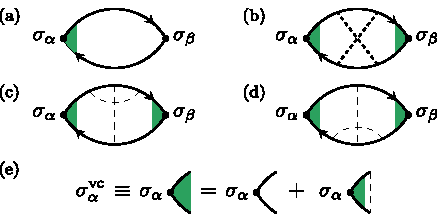
\includegraphics[]{articles/dirac_fm/fig2}
\caption{Diagrams considered in the calculation of $\hat{K}$: (a) non-crossing diagram, (b) $X$ diagram, (c-d) $\Psi$ diagrams. Green areas indicate the ladder summation (e) for the vertex correction in the non-crossing approximation \protect\cite{ivan}.}
\label{fig:diagrams}
\end{figure}

In our calculation the terms of the order of $\alpha \ln p_\textrm{cutoff}/\ep$ (where $p_\textrm{cutoff}$ is the ultraviolet momentum cut-off) is disregarded with respect to $1$. This approximation is legitimate since we assume that all model parameters $\epsilon$, $\Delta_\textrm{sd}$ and $\alpha$ are first renormalized such that $p_\textrm{cutoff} \approx \ep$.

It is, then, easy to see that the vertex-corrected spin operator is readily obtained from the geometric series of powers of $\pi\alpha \hat{M}$, 
\begin{align}
\sigma_\alpha^\text{vc} &= 
\sigma_\alpha+\pi\alpha \hat{M}_{\alpha\beta}\sigma_\beta+(\pi\alpha)^2 (\hat{M}^2)_{\alpha\beta}\sigma_\beta+\dots\nonumber\\
&=\left[1-\pi\alpha \hat{M}\right]^{-1}_{\alpha\beta}\sigma_\beta.
\end{align}
Thus, in the non-crossing approximation (illustrated in Fig.~\ref{fig:diagrams} (a)), one simply finds $\hat{K}= \hat{M}[1-\pi\alpha \hat{M}]^{-1}$. 